%Plantilla basada en "Template for Masters / Doctoral Thesis" (plantilla disponible en writeLaTex) que subió LaTeXTemplates.com

\documentclass[11pt]{book}
\usepackage[paperwidth=17cm, paperheight=22.5cm, bottom=2.5cm, right=2.5cm]{geometry}
\usepackage{amssymb,amsmath,amsthm} %paquete para símbolo matemáticos
\usepackage[spanish]{babel}
\usepackage[utf8]{inputenc} %Paquete para escribir acentos y otros símbolos directamente
% for inline and display quotations.
\usepackage[autostyle]{csquotes}
\usepackage{enumerate}
\usepackage{graphicx}
%\usepackage{subfig} %para poner subfiguras
\graphicspath{{Img/}} %En qué carpeta están las imágenes
\usepackage[nottoc]{tocbibind}
\usepackage[T1]{fontenc}
\usepackage{lmodern}
\usepackage{minted}
\usepackage[pdftex,
            pdfauthor={Dudley Esteban Díaz Suárez},
            pdftitle={Diseño de un Sistema de Procesamiento de Lenguaje Natural para la Atención a Clientes Automatizada},
            pdfsubject={ÁREA DE LA TESIS},
            pdfkeywords={PALABRAS CLAVE},
            pdfproducer={Latex con hyperref},
            pdfcreator={pdflatex}]{hyperref}
\usepackage{filecontents}




\begin{document}

\renewcommand{\proofname}{Demostración}
\providecommand{\norm}[1]{\lVert#1\rVert} %Provee el comando para producir una norma.
\providecommand{\innp}[1]{\langle#1\rangle} 
\newcommand{\seno}{\mathrm{sen}}
\newcommand{\diff}{\mathrm{d}}

%\newtheorem{teo}{Teorema}[section] 
%\newtheorem{cor}[teo]{Corolario}
%\newtheorem{lem}[teo]{Lema}

%\theoremstyle{definition}
%\newtheorem{dfn}[teo]{Definición}

%\theoremstyle{remark}
%\newtheorem{obs}[teo]{Observación}

%\allowdisplaybreaks


%----------------------------------------------------------------------------------------
%	PORTADA
%----------------------------------------------------------------------------------------

\title{Diseño de un Sistema de Procesamiento de Lenguaje Natural para la Atención a Clientes Automatizada} %Con este nombre se guardará el proyecto en writeLaTex

\begin{titlepage}
\begin{center}

\textsc{\Large Instituto Tecnológico Autónomo de México}\\[4em]

%Figura
\begin{figure}[h]
\begin{center}

\includegraphics{logo-ITAM_ch.jpg}
\end{center}
\end{figure}

\vspace{4em}

\textsc{\huge \textbf{Diseño de un Sistema de Procesamiento de Lenguaje Natural para la Atención a Clientes Automatizada}}\\[4em]

\textsc{\large Tesina}\\[1em]

\textsc{que para obtener el título de}\\[1em]

\textsc{INGENIERO EN COMPUTACIÓN}\\[1em]

\textsc{presenta}\\[1em]

\textsc{\Large Dudley Esteban Díaz Suárez}\\[1em]

\textsc{\large Asesor: DR. JOSÉ OCTAVIO GUTIÉRREZ GARCÍA}

\end{center}

\vspace*{\fill}
\textsc{México, D.F. \hspace*{\fill} 2018}

\end{titlepage}


%----------------------------------------------------------------------------------------
%	DECLARACIÓN
%----------------------------------------------------------------------------------------

\thispagestyle{empty}
\vspace*{\fill}
\begingroup
``Con fundamento en los artículos 21 y 27 de la Ley Federal del Derecho de Autor y como titular de los derechos moral y patrimonial de la obra titulada ``\textbf{Diseño de un Sistema de Procesamiento de Lenguaje Natural para la Atención a Clientes Automatizada}'', otorgo de manera gratuita y permanente al Instituto Tecnológico Autónomo de México y a la Biblioteca Raúl Bailléres Jr., la autorización para que fijen la obra en cualquier medio, incluido el electrónico, y la divulguen entre sus usuarios, profesores, estudiantes o terceras personas, sin que pueda percibir por tal divulgación una contraprestación''.

\centering

\hspace{3em}

\textsc{AUTOR}

\vspace{5em}

\rule[1em]{20em}{0.5pt} % Línea para la fecha

\textsc{Fecha}
 
\vspace{8em}

\rule[1em]{20em}{0.5pt} % Línea para la firma

\textsc{Firma}

\endgroup
\vspace*{\fill}


%----------------------------------------------------------------------------------------
%	DEDICATORIA
%----------------------------------------------------------------------------------------

\pagestyle{empty}
\frontmatter

\chapter*{}
\begin{flushright}
\textit{DEDICATORIA}
\end{flushright}


%----------------------------------------------------------------------------------------
%	AGRADECIMIENTOS
%----------------------------------------------------------------------------------------

\chapter*{Agradecimientos}
%\markboth{AGRADECIMIENTOS23}{AGRADECIMIENTOS} % encabezado 

¡Muchas gracias a todos!


%----------------------------------------------------------------------------------------
%	PREFACIO
%----------------------------------------------------------------------------------------

%\chapter*{Prefacio}

\pagestyle{plain}
%\markboth{PREFACIO23}{PREFACIO} % encabezado 

%PUEDEN QUITAR ESTA PARTE


%----------------------------------------------------------------------------------------
%	TABLA DE CONTENIDOS
%---------------------------------------------------------------------------------------

\tableofcontents


%----------------------------------------------------------------------------------------
%	TESIS
%----------------------------------------------------------------------------------------
\mainmatter %empieza la numeración de las páginas
\pagestyle{headings}

%  Incluye los capítulos en el folder de capítulos

\chapter{Introducción}

\textbf{Antecedentes}

A partir del uso cada vez más cotidiano de chat como medio de comunicación han surgido un gran número de plataformas de mensajería instantánea. Actualmente algunas empresas, sobre todo en Asia, han visto un aumento sustancial en ventas al usar plataformas como Line o Wechat para acercarse a sus clientes. Estos sistemas y plataformas han ido evolucionando y sofisticando su uso. A grado tal ha llegado la adopción del chat que para algunas empresas es la base de venta para todos sus productos.

Por un lado, a partir de la compra de Whatsapp por Facebook, se ha visto en la empresa californiana un interés sobre el uso de su plataforma de mensajería instantánea, Messenger, como plataforma para el contacto de empresas en Occidente. 
Desde la convención de desarrolladores de Facebook (F8) en 2016, donde anunciaron la apertura de su API para Messenger, se ha visto un constante crecimiento en el número de personas y empresas que quieren aprovechar a la gran base de usuarios que Facebook pone a su alcance.

Además existen trabajos que han demostrado que la automatización de flujos de adquisición de clientes es benéfico para empresas que buscan aumentar su base de clientes y ofrecer productos innovadores \cite{makar2014automatic}. Se considera que hay dos componentes principalmente front-end y back-end.\cite{patil2017comparative} Existen actualmente varias formas de crear un agente de este tipo y se compararán aquí más adelante. 

Por otro lado, Resuelve es una empresa cuya misión es ayudar a las personas a solucionar problemas financieros. Cuenta con más de 6 años de experiencia y sucursales por toda la República Mexicana y Colombia. Además de aproximadamente 1,600 colaboradores  Cuenta con varias líneas de negocio. Resuelve tu deuda es una reparadora de deuda y la línea de negocio más grande de la familia Resuelve. Para la  adquisición de clientes, el equipo de marketing en Resuelve, ha encontrado los medios digitales como la mejor vía. Actualmente  90\% de los clientes se enteraron de Resuelve tu deuda a partir de un anuncio de Adwords, Facebook o correo electrónico. Del 90\% de clientes aproximadamente el 50\% viene de Facebook, incluyendo anuncios pagados, página de admiradores (Fan pages) y conversaciones orgánicas. La parte de anuncios pagados se hace programáticamente, mientras que la parte conversacional es con personas que se dedican exclusivamente a responder dudas generales y hacer que dejen sus datos de contacto. 
Además de lo anterior se ha visto que aún siendo clientes, hay dudas sobre cómo van avanzando en algún proceso interno. Lo cual hace el número de personas que atienden a clientes sea insuficiente. Se ha calculado que para el número de clientes, actuales y proyectados, es incosteable tener un número mayor de personas atendiendo a clientes.  Lo que ocasiona baja calidad en el servicio, un malestar en los clientes, bajas de clientes, mala imagen y pérdidas económicas. 

Viendo la necesidad que se presenta y la apertura de plataformas como Facebook es que se propone en esta tesis es hacer un bot. El bot buscará dar respuestas automáticas a clientes o prospectos que buscan información o que estén interesados en el programa de reparación de deuda.

\textbf{Objetivo}

Este proyecto tiene como objetivo llevar a cabo la creación de un chatbot para la adquisición de clientes automática a partir de interacciones en Facebook Messenger.

\textbf{Requerimientos funcionales}

El proyecto tiene como alcance crear un chatbot que pueda tener una conversación guiada por menús, botones, respuestas rápidas e introducción de texto con personas que accedan a la conversación de Resuelve Tu Deuda a través de Facebook Messenger. Existirá una opción para saber más información, donde el usuario responderá con sus datos de contacto a las preguntas planteadas. Los datos de contacto serán almacenados en una base de datos, donde se almacenan los datos de todos los usuarios con interés en el producto.

\textbf{Restricciones}

La empresa estaba bajo el uso de herramientas del ecosistema de Amazon Web Services, así que cualquier desarrollo tendría que ser compatible con estas herramientas
Como plataforma de mensajería instantánea se debe utilizar Messenger o Whatsapp
El desarrollo, puesta en producción y operación del bot tiene que ser de bajo costo. Lo cual implica que entre todos los costos de operación, sin incluir el sueldo de las personas que desarrollan y mantienen el bot, debe ser el costo de adquisición por cliente menor al de la adquisición unitaria de clientes por otros canales digitales. Es decir, un lead del bot debe costar menos que un lead de canales como Facebook Ads, Adwords o un proveedor de leads externo.
El chatbot debe estar optimizado para tener más clientes.

\textbf{Alcance}

Se desea crear un chatbot que sea capaz de interactuar con posibles clientes en la plataforma de Facebook Messenger. Las interacciones tendrán como objetivo dar información sobre el servicio que Resuelve Tu Deuda ofrece y también de pedir los datos de personas interesadas en adquirir el servicio de reparación de deuda. El sistema será capaz de recopilar esta información y guardarla en el sistema de administración de clientes o CRM (por sus siglas en inglés) para sus seguimiento por el área de ventas. Adicionalmente debe tener la capacidad de tener un sistema de análisis de interacciones y emisión de notas que vengan del blog de la empresa a múltiples segmentos de usuarios. El sistema debe estar activo todo el día y todos los días. Así mismo, si es necesario un usuario puede pedir la asistencia de una persona que le de información más detallada de su situación.

\textbf{Justificación}

La teoría nos indica que a partir de una buena planeación es más probable que lleguemos al éxito. Es por eso que lo primero que se pensó hacer en este proyecto fue definir para qué se quería tener un chatbot. Las razones principales de la implementación debían referir a la pregunta ¿Tener un chatbot mejora en algún sentido el producto que ofrecemos? Ya que un bot, un chatbot en este caso, aunque puede parecer un medio/producto innovador para los más entusiastas de la tecnología; no necesariamente sería algo que pueda interesar al cliente objetivo del negocio.


Se sabe que el uso de tecnología para comunicarnos se ha adoptado cada vez más en los recientes años y según investigaciones de Facebook se sabe que el chat es medio de contacto preferido para la generación actual y hasta dos generaciones anteriores \cite{moremessage2016}. Ya que les parece un medio rápido y práctico de estar en contacto. Viendo esto se sabe que tenemos la oportunidad de mejorar el contacto con usuarios en donde más les agrada comunicarse.

El primer objetivo, se centra en aumentar la obtención de clientes y el segundo mejorar el servicio de post-venta. Se definen estos objetivos por varias razones:

El primero es muy sencillo, entre más clientes, mayores utilidades para la empresa. Esto aunado a la baja del costo por obtención de cliente y aumento en la probabilidad de cierre de venta. El costo de obtener los datos de un prospecto a cliente depende de varios factores:


Existen canales adicionales (expos, radio, TV, espectaculares), los cuales no son muy efectivos en volumen de leads\cite{wiki:leadgen2018}, pero son de muy buena calidad, ya que casi todas las personas que se enteran desde esos medios y nos dan sus datos de contacto tienen un porcentaje de conversión a cliente (Porcentaje de Fase 2 (\% F2) mayor a 60\%. El chatbot debería poder presentarse aquí como una ayuda para responder preguntas más puntuales, seguir la conversación y permitirle al prospecto dejar sus datos.
El chatbot se propone como un canal alterno también. Donde cualquiera que tenga dudas o tenga el interés puede dejar sus datos y se le dará seguimiento a su caso. En cualquier sentido el costo de operación debería ser muy bajo para que no aumente en demasía el dinero invertido en los demás canales de adquisición de clientes.

La probabilidad de cierre reside en la hipótesis: a mejor interacción e información tenga el prospecto, será más sencillo convencerlo de comprar en el momento de la venta. El chatbot debería poder cumplir con el aumento de información proporcionada con una interacción amigable.

El segundo objetivo es mejorar el servicio al cliente a través de la tecnología. Al crecer la empresa el número de clientes que tiene dudas diversas sobre el producto aumenta. Y ha aumentado a tal grado que un agente de servicio a cliente llega a tener hasta 600 personas a las que tiene que atender. Esto hace que disminuya la calidad de seguimiento que un cliente necesita, lo cual resulta en descontento y en el peor de los casos baja definitiva del programa.

\textbf{Metodología}
Se hará una investigación sobre el estado actual de los chatbots actuales y cuales son sus usos. A partir de esto se clasificará y elegirá el tipo de chatbot que es necesario para lograr el objetivo. 
Después, se preguntará a las área de Ventas, Marketing y Servicio a Cliente acerca del acercamiento y trato a clientes institucional. 
Enseguida, se hará un borrador de conversación guiada, el cual tendrá como objetivo sentar la estructura del chatbot. A partir de la estructura se creará el contenido de las interacciones, para crear el flujo en la herramienta y que quede implementado para la interacción de clientes.
Por último, se integrará al flujo de creación de leads de la empresa. Se harán pruebas para asegurarse que todos los elementos del sistema funcionen correctamente y pruebas de concepto con usuarios internos. Se harán los cambios necesarios según sean necesarios. Se abrirá al público y se promocionará con anuncios pagados en la plataforma de anuncios de Facebook. Al finalizar, se hará un análisis de costos para descubrir si la adquisición de clientes es más rentable a partir de la integración del chatbot.

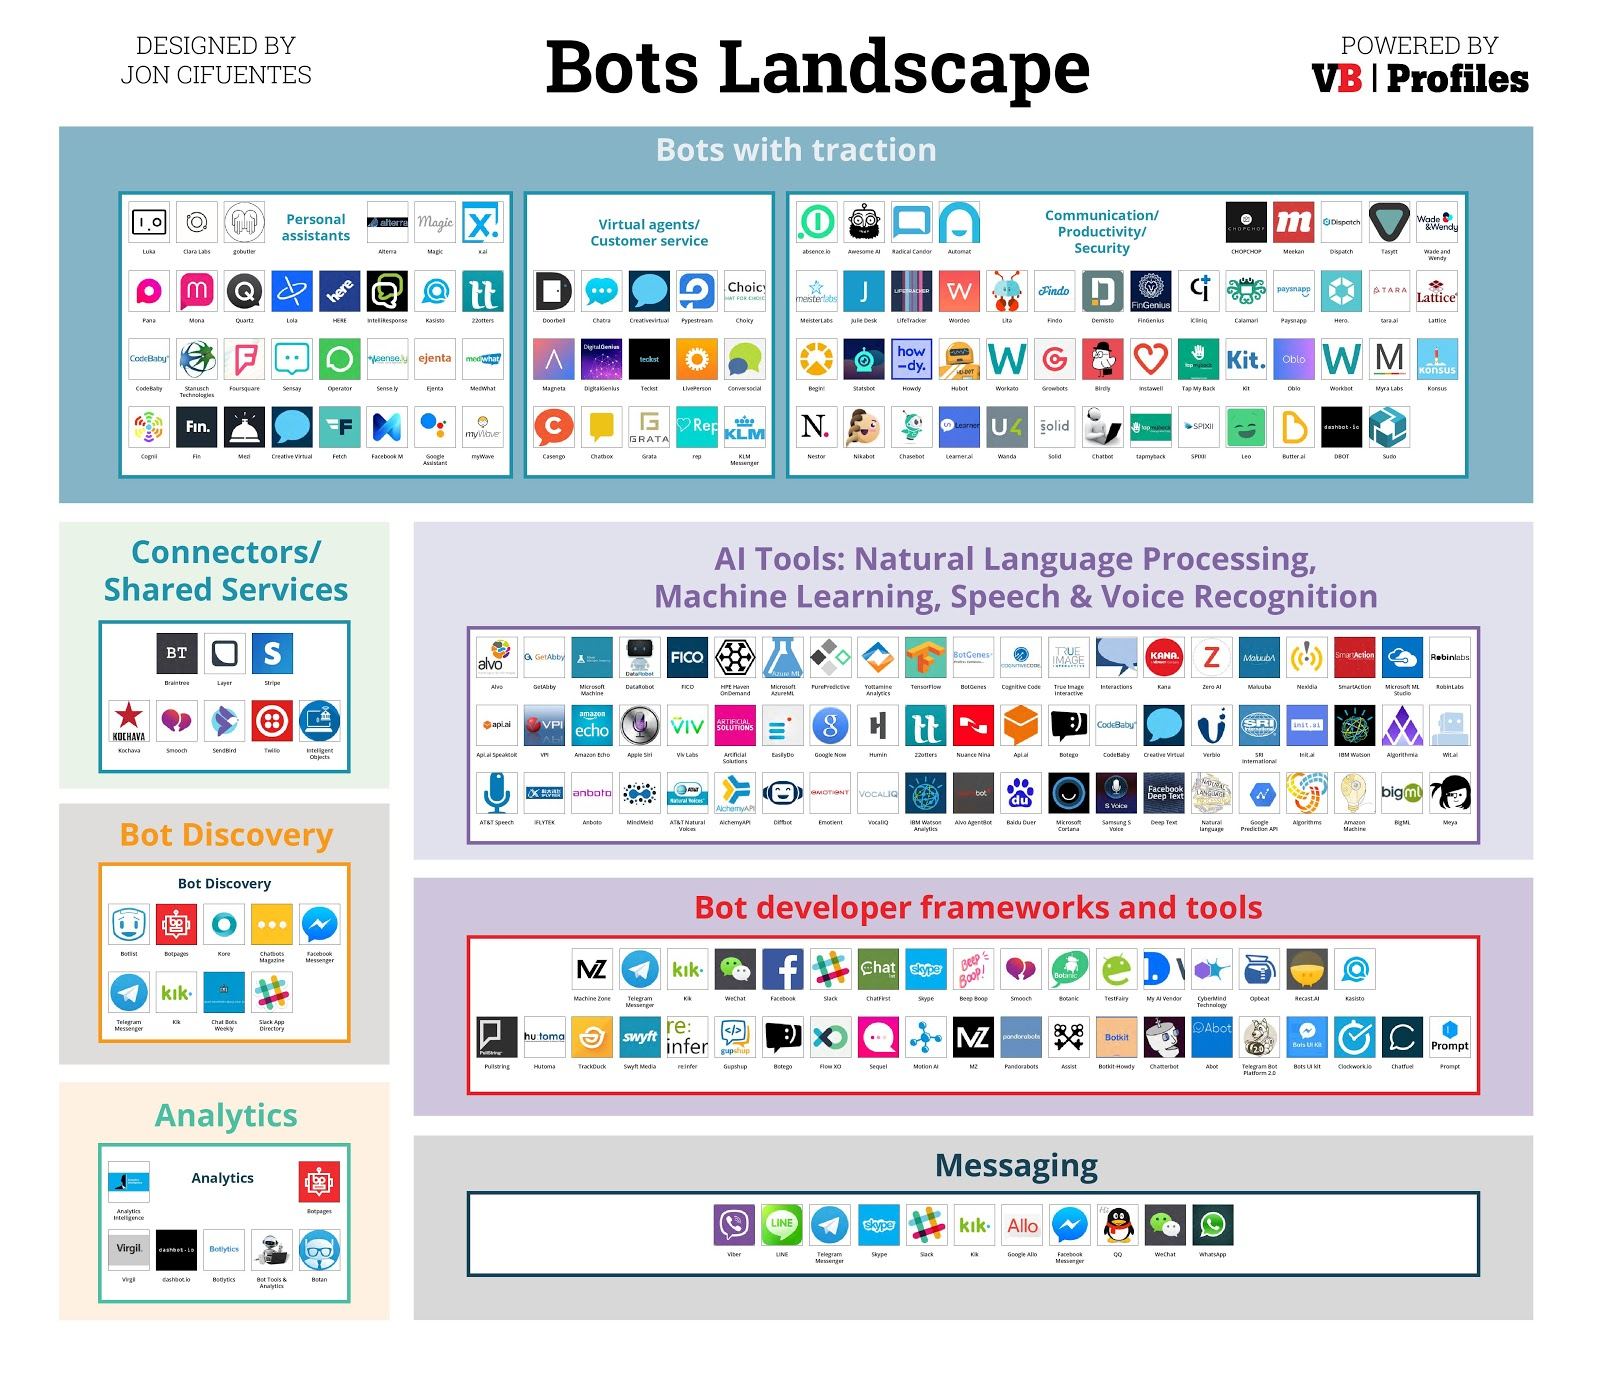
\includegraphics[width=\textwidth]{PanoramaBots.jpg}


\chapter{Marco Teórico}

\textbf{Soluciones alternas}
Hacer un chatbot es una solución a un problema que ya estaba siendo atendido, pero que se quería atacar de forma diferente. Sin embargo, queda lejos de ser la única solución al problema de la interacción con clientes a través del chat de Facebook Messenger. Hablemos de algunas de las soluciones alternas a este problema.

 Empezando por cómo se venía haciendo tradicionalmente. El chat de Resuelve tu deuda era atendido únicamente por una persona, que se dedicaba a estar al pendiente de lo que los prospectos y clientes querían comunicar (Dudas, aclaraciones, comentarios, etc). Esta persona tenía que estar todo el día atenta al servicio de estas personas y contestarles acorde a sus mensajes. 

Esta forma de interacción era adecuada para los usuarios, ya que podían recibir la respuesta adecuada la mayoría de las veces. Sin embargo tiene sus contras. Al ser una persona la que contesta, el tiempo que le dedica a una conversación es limitado y solo puede atender una conversación a la vez; así como el horario en el que puede contestar. Sin mencionar que todo el conocimiento está centralizado en la privacidad del cerebro del community manager, el cual al irse de la empresa se lo lleva y se tiene que entrenar a otra persona. Tanto a lo que se les contesta a los usuarios como la forma en que se les contesta. Aunque este punto puede ser mejorado haciendo una base de conocimiento (la cual, hasta el momento de hacer este bot, no existe), el entrenamiento de una persona sigue siendo un problema latente. Dicho lo anterior se nota que es mejorable este tipo de interacción. 

Otra posible solución es la de crear un app móvil. Esta solución tiene varios puntos a favor, como que siempre esté disponible una respuesta a un usuario, el tono y contenido del mensaje vayan acorde a los que maneja la empresa y que no nos tenemos que preocupar por que el app vaya a ser despedida o renunciar. 

Sin embargo, es muy poco probable que alguien descargue un app para solucionar preguntas de un servicio del cual no es usuario. Para solucionar el tema de descargar un app móvil se podría pensar en hacer una webapp. Un sistema cuya interacción se a través de un navegador web, el cual se encuentra en cualquier dispositivo móvil y computadora. Aún resolviendo esta barrera de acceso, lo invertido en un app web/móvil puede llegar a ser mucho dinero, tiempo y esfuerzo (añadir referencia de lo que cuesta hacer un app).  Entonces, esta solución tampoco suena tan coherente para el problema en cuestión.


Algunas compañías, sobre todo del tipo Saas, utilizan algo llamado base de conocimiento (o knowledge base). La cual funge como una gran página de FAQs (preguntas frecuentes), donde se ponen las preguntas con respuestas más frecuentes y ‘obvias’ que los cliente han tenido o pueden tener. Este enfoque es más de autoservicio y evita tener a una persona respondiendo individualmente a cada usuario. Sin embargo, estas preguntas se van haciendo como vayan siendo necesarias y existe el riesgo de que haya inconsistencia y preguntas repetidas. También esto implica tener que estar buscando las preguntas, lo cual es más laborioso para el usuario y fácilmente puede ya no querer seguir en el sitio.

Podemos ver como todas las soluciones tienen ventajas, sin embargo hay algunas  desventajas que nos hacen ver que otro tipo de interacción sería mejor. Como la de un chatbot. Un chatbot está pensado para estar disponible siempre, no se enferma y si no funciona como queremos lo podemos mejorar, sin tener que lidiar con personas. La base de conocimiento puede ser ampliada y se guarda en un lugar para su continua mejora. El medio de contacto es en el chat de Facebook Messenger, lo cual resulta muy conveniente, porque no requiere que el usuario tenga que cambiar de programa o descargar una nueva app. Otra ventaja que se asume es que el usuario ya está familiarizado con el uso de un chat. Según datos de Facebook hay 1,200 millones de personas que usan su Messenger alrededor del mundo. \cite{zuckerberg2017results}


Teniendo una base tan grande de usuarios y considerando que México es uno de los 5 países con más usuarios en Facebook debería ser muy sencillo interactuar con el bot dentro de esta plataforma.

\textbf{Tipos de chatbots}

Un bot conversacional o chatbot es un programa que busca simular una conversación a partir de la entradas hechas por un usuario. Usualmente las entradas son en forma de texto, aunque también hay algunos que aceptan entradas de otro tipo, como la voz. Aquí nos centraremos en los que solo interactúan a través de entradas de texto. Aunque parece ser muy reciente la creación de chatbots, se sabe que desde los años 50 existían algunos, como Eliza, que trataban de imitar la conversación de una persona y pasar la prueba de Turing. Actualmente existen muchos chatbots en el mercado con una gran variedad de usos. Se clasifican de diferente maneras. La que usaremos es partir de la propuesta que nos ofrece el investigador Dotan Elharrar Product Manager en Microsoft AI and Research a partir de las funciones que tienen y el valor que proveen al usuario:

\textbf{Optimizador}
Este tipo de bot trata de resolver cierta tarea mejor que cualquier opción ya existente, se un app, un sitio web, un programa, etc. 
Un ejemplo de esto es decirle a un sistema como Siri en un dispositivo iOS que reproduzca una canción y no tener que desbloquearlo, abrir la aplicación, buscar la a canción, encontrarla y reproducirla. Este asistente usa una interfaz de lenguaje natural por voz para poder responder preguntas que en su mayoría serán delegadas a servicios en Internet como Wikipedia, el buscador de Google o algún app nativa.
\textbf{Mono-utilitario}
Son bots que tienen una sola pequeña función utilitaria o lúdica y que cuentan con una interfaz de chat. Algunos de los ejemplos son bots que permiten hacer de una imagen un meme o un texto en un video.
Tal es el caso de \textit{Erwin} \cite{niefelderwin2017}, un chatbot cuya finalidad es de proveer acertijos y validar las respuestas introducidas. O el bot de \textit{La prueba de Rorschart} \cite{niefeldrorschach2017}, cuyo fin es conocer aspectos de la personalidad de una persona a mostrándole imágenes con manchas de tinta.
\textbf{Proactivo}
Bots que pueden dar información muy útil en casos muy concretos. Sin embargo, para interacción en una situación cotidiana no tienen utilidad. 
Un ejemplo es el bot de KLM \cite{klm2016messenger}, que le ayuda a los pasajeros de la aerolínea a recordar sus vuelos, dar avisos de cambios de itinerario, tener digitalmente sus boletos y cambiar detalles de su viaje. Sobre todo funciona para seguir en contacto con sus clientes y ver hábitos de consumo para hacer una mejor segmentación y análisis
\textbf{Social}
Este es un tipo de bot que suele ser muy parecido al mono-utilitario, sin embargo cuenta con dos características que lo separan: se basa en la interacción social y da lugar a la multitud para que sea la voz principal de la conversación. Funge sólo como guía de la conversación. Ejemplo de esto es \textit{Swelly} \cite{swelly2017messenger}. 
Swelly es un chatbot que ayuda a gente que quiere decidir ante dos posibilidades. i.e. Dos vestidos, dos lugares a donde ir, dos tipos de comida,etc. Esta información es recopilada y se le manda a la persona que preguntó lo que la comunidad ha elegido.

\textbf{Escudo}
Estos bots son creados para evitar que tengamos malas experiencias. Se parecen a los optimizadores sin embargo tratan de evitar que tengamos platicas con un humano cuando una máquina podría solucionarnos el problema fácilmente. Ejemplos de esto son el agente virtual de servicio a cliente de Microsoft o \textit{DoNotPay} \cite{donotpay2017} el chatbot que te ayuda a apelar multas de tránsito.
\textbf{Conversacional}
Este tipo de bots están dedicados solo a entablar una conversación con el usuario. Se usan principalmente como método de investigación y retención de usuario. Tener una conversación puede parecer entretenido y se cree que al interactuar con este tipo de bots se puede conocer a una persona de una mejor manera. Ejemplo de este tipo de bots es \textit{Xiaoice} \cite{wiki:Xiaonic} , un chatbot que hace las veces de una niña de 12 años, la cual principal objetivo es entablar una conversaciones. Ha tenido más de 10 mil millones de conversaciones y puede considerarse como la prueba de Turing más larga de la historia.
Asistente personal
Este tipo de bots tienen múltiples funcionalidades y han evolucionado al punto de ser plataformas para la ejecución de programas y  bots de menor funcionalidad. Algunos son capaces de tener entradas de voz inclusive. Algunos ejemplos son los asistentes personales como Siri de Apple, Cortana de Microsoft, Allo y Google now de Google. Así como un desarrollo de la universidas Metropolitana de Manchester, \textit{Betty} \cite{curry2013betty}.


\textbf{Panorama actual de los chatbots}

 Desde 1960 con LIZA\cite{shawar2005using}, hasta 2018 con productos como Siri o Google Now, el panorama de los chatbot ha ido evolucionando y haciéndose más complejo. Se puede observar en el diagrama a continuación la amplia gama piezas que pueden intervenir en un bot conversacional actual.



%\thispagestyle{empty}
\chapter{Investgación Interna}

Para saber más acerca del trato a clientes se tomó la iniciativa de preguntar a las áreas de ventas, servicio al cliente y administradores de comunidades de mercadotecnia , que dudas tienen los clientes, qué estrategias de ventas utilizan para cerrar una venta y cómo es el trato a clientes con dudas específicas.
Ya que la venta es a través del teléfono también se le pidió a los asesores que permitieran oír sus llamadas y así tener de primera mano la estrategia de venta del producto.

\textbf{Ventas}

Se le pidió a un equipo de asesores que tienen trato directo su opinión acerca de cuáles eran las dudas más frecuentes y el interés que tiene la gente en el programa de reparación de crédito. 
Lo que compartieron fue que los clientes tienen dudas sobre varias cosas:

\begin{itemize}
\item ¿Qué es buró de crédito?
\item ¿Cómo funciona la reparación del buró de crédito?
\item ¿Puede demandarlos una institución de crédito?
\item ¿Cuánto pagarían uniéndose al programa?
\item 
\end{itemize}

Oyendo las llamadas a clientes se pueden identificar varias cosas:
Son personas que están desesperadas por salir de deudas
La mayoría tiene deudas bancarias
Tienen casi todos las mismas preguntas y dudas:

\begin{itemize}
\item ¿Sirve el programa?
\item  ¿Es una empresa seria?
\item ¿Si me pueden ayudar a salir de deudas?
\item ¿Cuál es el proceso?
\item ¿Tiene costo?
\item 
\end{itemize}


\textbf{Servicio a Cliente}

Una de las áreas de oportunidad de la reparadora de deuda más grandes es el servicio a cliente. Existe una baja importante en el programa de reparación de crédito. El bot, aunque tiene como objetivo principal la adquisición de clientes, se quiere aprovechar para la retención en el programa.
Hablando con agentes de servicio a cliente y oyendo llamadas de clientes ya en el programa se encontraron varios puntos a resaltar:


\begin{itemize}
\item No entienden por qué no se han liquidado sus deudas
\item Están molestos porque siguen recibiendo llamadas de cobranza
\item No entienden las cuotas que implican estar en el programa
\item No comprenden la importancia de seguir el proceso y las repercusiones de salirse del programa
\item Se les olvida abonar a su cuenta para pagar sus deudas
\end{itemize}


\textbf{Community Managers}

Community managers son las personas encargadas de estar al pendiente de la presencia de la empresa en redes sociales. Entre sus actividades están publicar contenido para atraer a personas a conocer la marca, realizar dinámicas y concursos que den difusión al producto, revisar la reacción de la gente en los perfiles sociales, contestar a comentarios y hablar a través de chat para dar mayor información. El bot toma el lugar de las community manager como herramienta para eficientar el camino hacia la conversión del prospecto en el chat de Facebook Messenger. 
Hablando con la community manager de Resuelve tu deuda y leyendo 100 conversaciones escogidas al azar del año 2016, se observa que las personas interesadas tienen varias dudas:

\begin{itemize}
\item ¿Cómo funciona el programa?
\item ¿Funciona el programa?
\item ¿ A quién han ayudado?
\item ¿Cuales son las condiciones para poder entrar al programa? (monto de deuda, instituciones bancarias, atraso de deuda)
\item ¿Cuanto cobra Resuelve para entrar al programa?
\end{itemize}


\textbf{Estándares}
\begin{itemize}
\item HTTP/S
\item JSON
\end{itemize}


\chapter{Estructura y estrategia del bot}

Tomando en cuenta la investigación que se hizo con las área del capítulo anterior, y pensando en el tipo de bot que mejor podría satisfacer las áreas de oportunidad de la reparadora, se estructuró un chatbot.
Tomando en cuenta la clasificación que hace Elharrar \cite{elharrar_2017} podemos observar que queremos un bot que tenga varias dimensiones. Por un lado sería un bot \textbf{optimizador}, por su capacidad de resolver dejar tus datos mejor que en una página web o teniendo a una persona que capture tus datos; escudo, porque debería poder solucionar las dudas que la mayoría de las personas tienen sin tener que buscarlas por internet o preguntarle a una persona  y \textbf{proactivo}, ya que te sugiere y da información que solo te va a servir muy bien si quieres resolver tus deudas

\textbf{Descubrimiento}

Para que el bot sea usado tiene que ser descubierto, por ello se proponen algunas estrategias:
\begin{itemize}
\item Poner el botón de messenger directamente en cualquier parte del dominio de la empresa y en la FanPage.
\item Messenger permite el escaneo de códigos de perfil que llevan directamente a una conversación del bot. Poner el código impreso en stands de  ferias, exposiciones y eventos presenciales y que se direccionen a los interesados directamente a Messenger y al bot.
\item Hacer campañas de anuncios pagados que dirijan directamente a la conversación de Messenger
\item 
\end{itemize}

\textbf{Introducción a la aplicación}

Al iniciar la aplicación existen 3 herramientas:

\textbf{-Saludo}
La primera vez que la persona entra a la conversación le puedes explicar el motivo de la conversación, el modo de comunicación y un resumen sobre el tema a tratar (hasta 180 caracteres). Se queda hasta arriba y no aparece más.

Se explicar muy resumido de lo que trata Resuelve y que vamos a contestar dudas generales en esta conversación.

\textbf{-Botón de inicio}

 Es un claro call-to-action para el usuario e indica al bot que se inicia la conversación. Lo ideal es poner un mensaje acorde al contexto (saludo)

\textbf{-Mensaje de Bienvenida}

Aquí se puede especificar que esta conversación es para aclarar dudas generales y tomar datos para prospectos. En iteraciones futuras puede explicarse que puede fungir como un centro de noticias financieras si nos dan la oportunidad. Podemos ser menos genéricos poniendo el nombre de la persona y a lo mejor algún otro dato relevante (según la hora del día dar un saludo diferente)
Hay que tener en cuenta que cada que vaya mejorando el bot habrá que cambiar este saludo para dejar en claro expectativas y capacidades.

\textbf{Interacciones}

En la primera iteración se tendrán mensajes que incluyan texto, imágenes y botones.

Se tratará que el flujo de la conversación sea dirigido por los mensajes interactivos, poniendo las preguntas en el cuerpo del mensaje y las respuestas disponibles hasta abajo del mismo.

Se contempla usar el template genérico.

Se debe tomar en cuenta la consistencia entre mensajes, no mezclar diferentes tipos de mensaje en una respuesta y ser lo más concisos sin dejar información incompleta.

\textbf{Callbacks}

Se configurarán callbacks para registrar eventos clave en GA:

- Interés en el programa
- Inicia inserción de datos
- Termina inserción de datos
- Pide una persona para que lo asista


Al momento de tener datos de contacto se deben mandar los mismos al CRM o alguna BD intermedia.

Se debe tomar en cuenta poner una respuesta una vez que se haga un callback sobre inserción de datos o algún otro callback para que la interacción sea más fluida y mejor la experiencia.
Utilizar más de un botón como opción en un callback, ya que pueden haber errores de inserción que el usuario no le estén dando la capacidad de cambiar.

\textbf{Actualizaciones y Alertas}

Una vez tomados los datos se puede seguir la interacción con contenido relevante (¿Cómo evitar deudas?, Tips diarios, etc.)

Es importante dar la opción para mandar este contenido y dejar en claro que es opcional. Se debería poder elegir la periodicidad de estas alertas y contenidos.
Si el tipo de contenido cambia se debe de notificar para que se de la aprobación necesaria.

Este tipo de notificaciones son una buena herramienta para tener más presente a la marca. Se puede hacer en otra iteración alertas personalizadas para hacer recordatorios de los días de pago o mandarlos como archivos de calendario al cerrar al cliente.

Se debe tener en cuenta no mandar demasiados para no saturar al cliente y que eso desencadene el desuso de la herramienta.

\textbf{Estados de Fallo}

Cuando se encuentre el bot en un estado donde falle o no sepa cómo contestar ser muy claro sobre ello. Tener algún mensaje para decirle a la persona que no se le entendió y que se puede comunicar de otra manera (botones, comandos).
Tener alguna opción para pedir asistencia humana en el último de los casos.
Mandar alertas sobre estados de fallo personalizadas y mejorar la experiencia con esos datos.
No hay que esperar perfección estudiar la interacción de los usuarios y descubrir qué puntos de frustración se pueden sanear.
Se recomienda dar mensajes de fallo variados para mantener la frescura y el gancho en la conversación.

\textbf{Lenguaje}

Aunque los chatbots sean medios automatizados innovadores no se debe perder el foco sobre a quién le hablamos. Debido a lo visto sobre la edad del grueso de clientes y el tipo de servicio ofrecido, se debe tener una comunicación semi-formal, pero que de confianza y sea muy informativa.

Es de gran importancia tomar un tono y mantenerlo durante toda la conversación.

Recordar que es un muy buen lugar para hacer familiares términos que pueden hacer más sencilla la asociación positiva de la marca y dar un mensaje de confianza. Se puede decir los beneficios que se tiene con Resuelve sobre hacer negociaciones por cuenta propia, explicar que todos los que hemos tenido préstamos estamos en buró de crédito y que resuelve ayuda a sanearlo y mejorar la calificación del cliente.

Tratar de ser lo más descriptivos en el objetivo de la conversación y los límites de la herramienta. Decir en qué parte del proceso se encuentran, qué entregables se esperan/pueden dar.

\textbf{Escribir las interacciones}

Hay que pensar en el flujo principal de la conversación y de ahí pensar en todas las posibles rutas que pueden seguir en la conversación.

En la primer iteración debería de ser muy guiado el flujo de la conversación y se debe ver como un árbol de decisión donde el usuario va navegando. Posiblemente al finalizar alguna rama regresar a alguna pregunta más general para que pueda tomar otra línea la conversación.

Tratar de tener varias formas de responder a una pregunta en pro de mantener la frescura de la conversación.

\textbf{Grafo de interacción guiada}

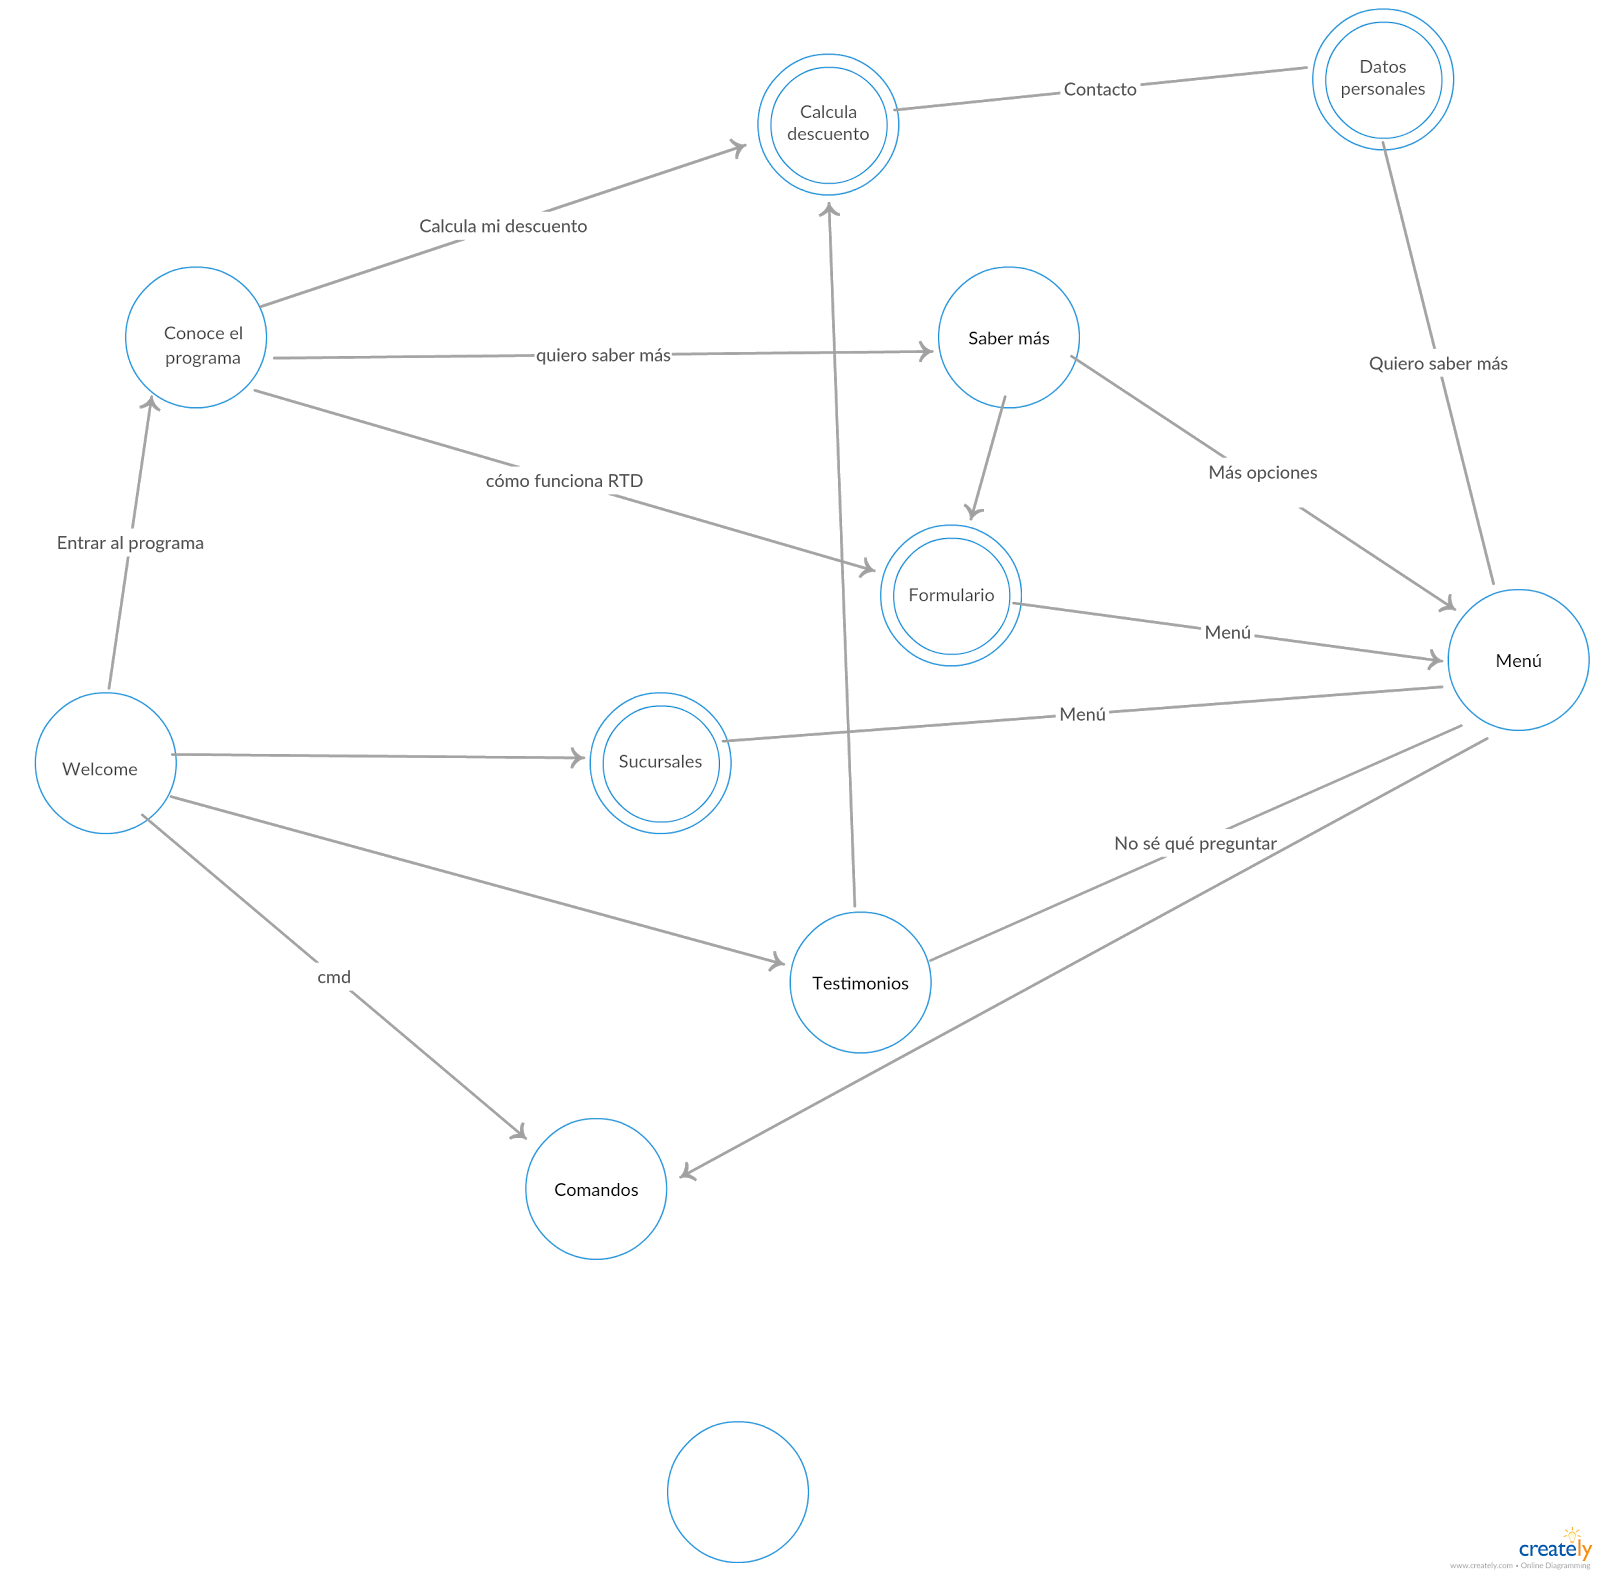
\includegraphics[width=\textwidth]{grafoInteraccion.jpg}

\chapter{Implementación}

\textbf{Plataforma de desarrollo}

Para construir el sistema se eligió Chatfuel \cite{sarinho2017splimbo} como herramienta de desarrollo. Esta herramienta está basada en bloques de contenido. Un bloque puede tener varios contenidos o tarjetas:
\begin{itemize}
\item Texto
\item Imágen
\item Galería de imágenes
\item Respuestas rápidas
\item Plugins:
\begin{itemize}
	\item API JSON, entrada de texto del usuario, crear variables de usuario, ir a bloque, Zapier, entre otras.
\end{itemize}
\end{itemize}

Las ventajas que esta plataforma ofrece son varias:
\begin{itemize}
\item Creación gráfica de bloques de contenido
\item Creación de la lógica entre bloques
\item Publicación automática a Facebook
\item Portabilidad a otras plataformas (Facebook Messenger, Telegram y próximamente Whatsapp, Kik y Slack)
\item Integración con plataformas de análisis
\end{itemize}

\textbf{Bloques de contenido}
A partir del uso de esta herramienta se construyeron los bloques de contenido. Los bloques se dividen en varias categorías:
Default - Aquí se define el saludo de bienvenida y la respuesta por defecto cuando la entrada de texto no se reconoce

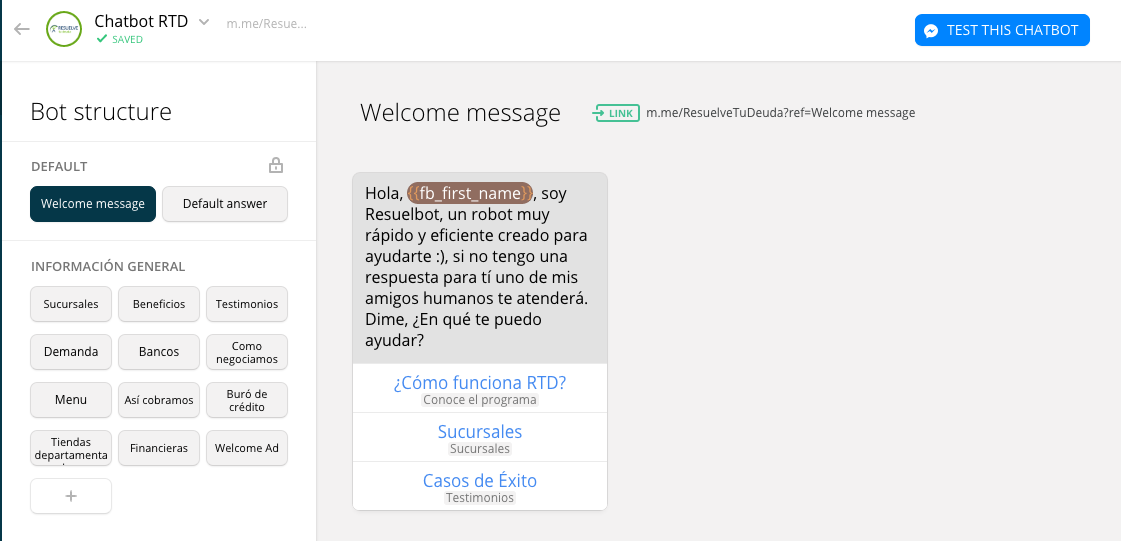
\includegraphics[width=\textwidth]{chatfuelWelcome.jpg}

Información General -  Aquí se da información de la empresa como sucursales, beneficios y testimonios; para aumentar la confianza del cliente sobre la reparadora de crédito.

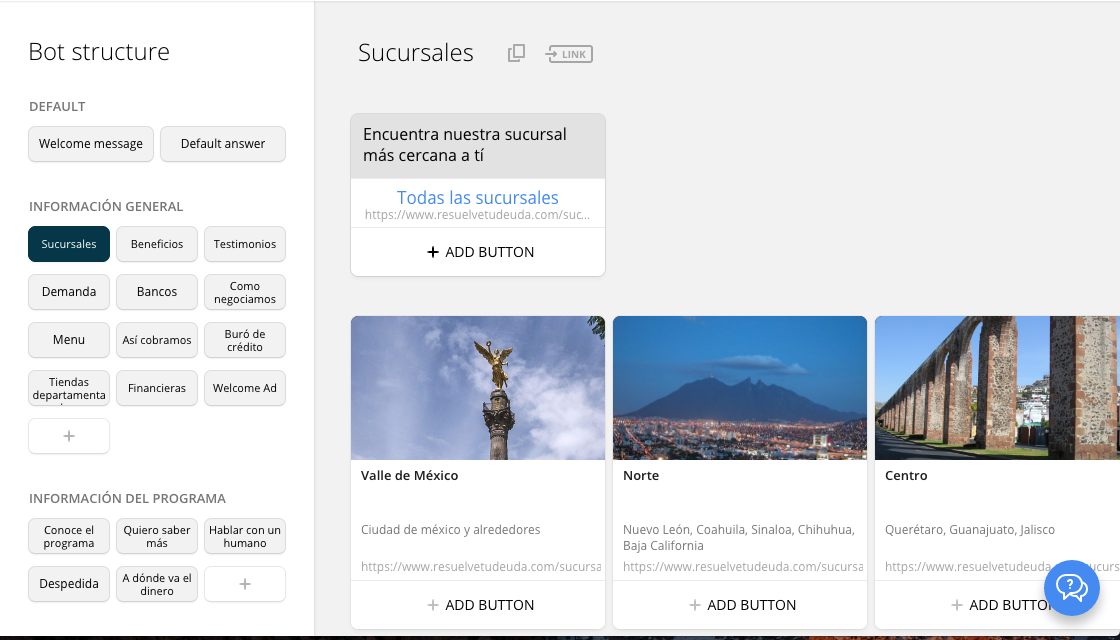
\includegraphics[width=\textwidth]{chatfuelSucursales.jpg}

Información del programa - Información general para conocer el programa de reparación de crédito

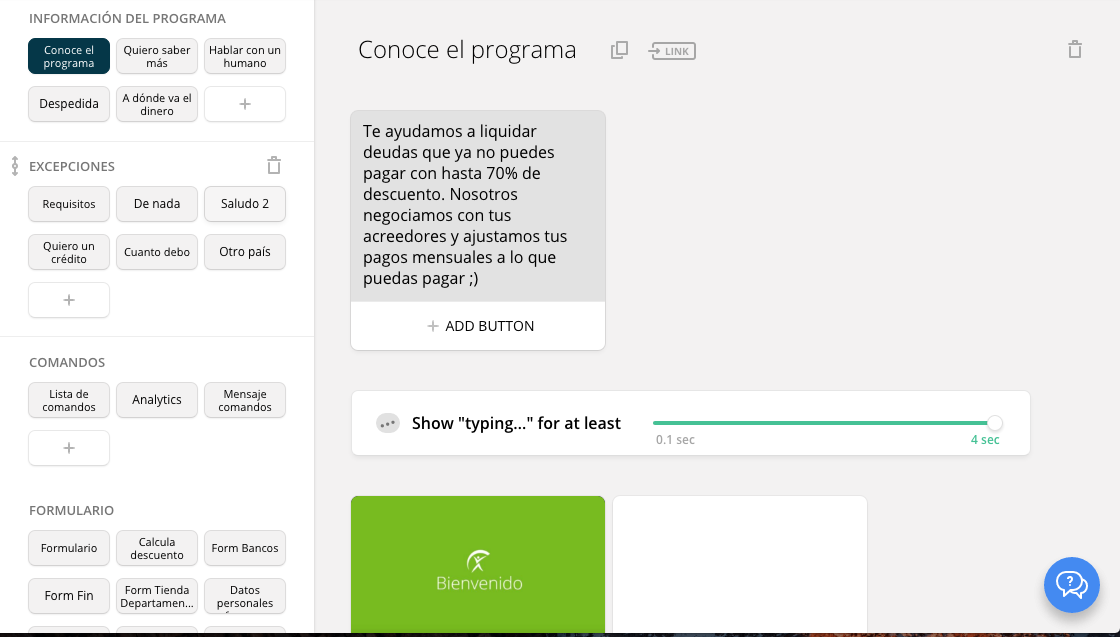
\includegraphics[width=\textwidth]{chatfuelConoceElPrograma.jpg}

Excepciones - Para algunos flujos, como el de cotización de descuento, existen requisitos (mínimo \$35,000 de deuda acumulada, ciertos bancos, etc). Si no se cubren los requisitos se muestra una excepción general de ese flujo explicando los requerimientos mínimos.

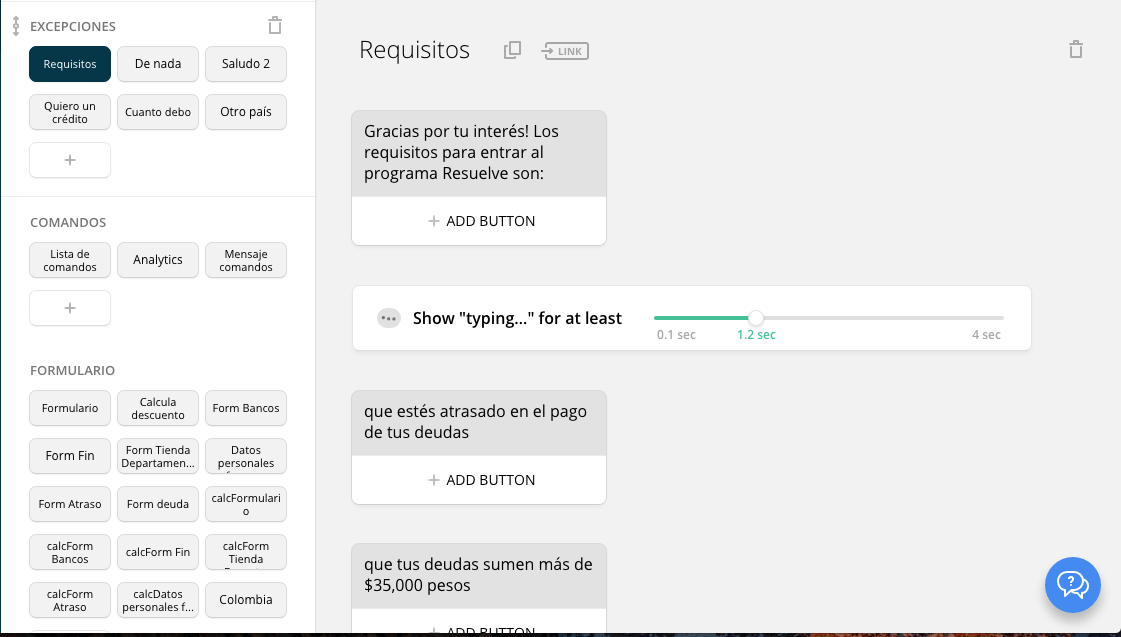
\includegraphics[width=\textwidth]{chatfuelRequisitosExep.jpg}

Comandos - La intención de este bloque es dar a conocer las funcionalidades que no son evidentes en la conversación y los detonadores que inician diferentes tipos de conversaciones.

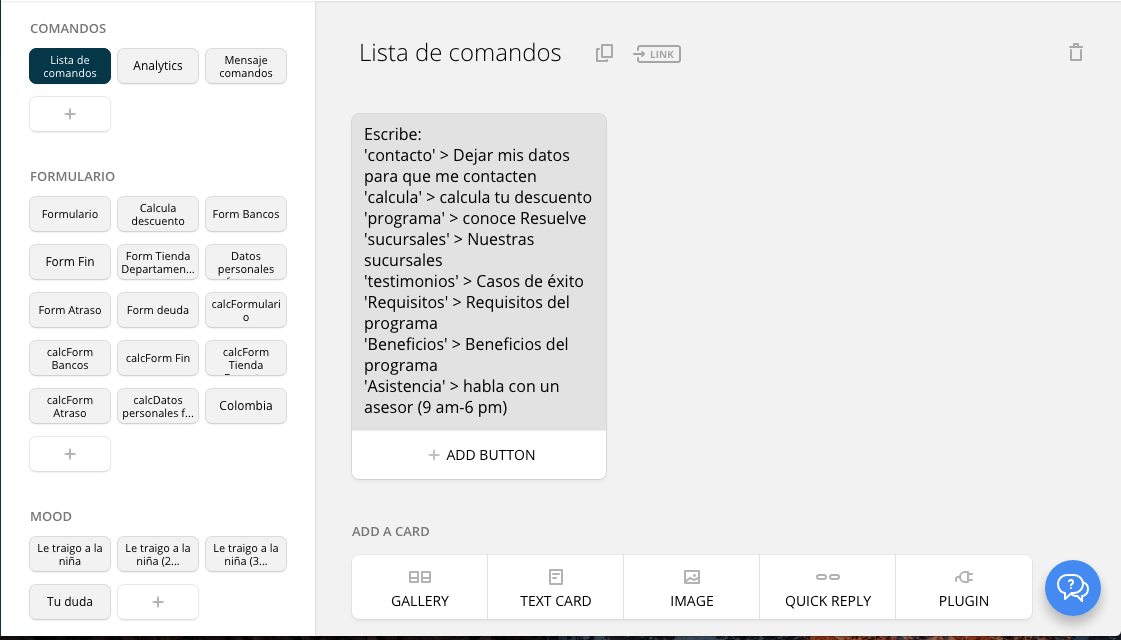
\includegraphics[width=\textwidth]{chatfuelComandos.jpg}

Anuncios de Facebook - Uno de los canales que más tráfico atrae es el de anuncios pagados en Facebook. Para poder medir el impacto de las campañas utilizadas se crearon el mismo número de bloques como campañas. En estos bloques se instancia el valor de la campaña de la que viene el usuario y se envía al final junto con los datos de contacto, si resulta en un lead, a la base de datos.

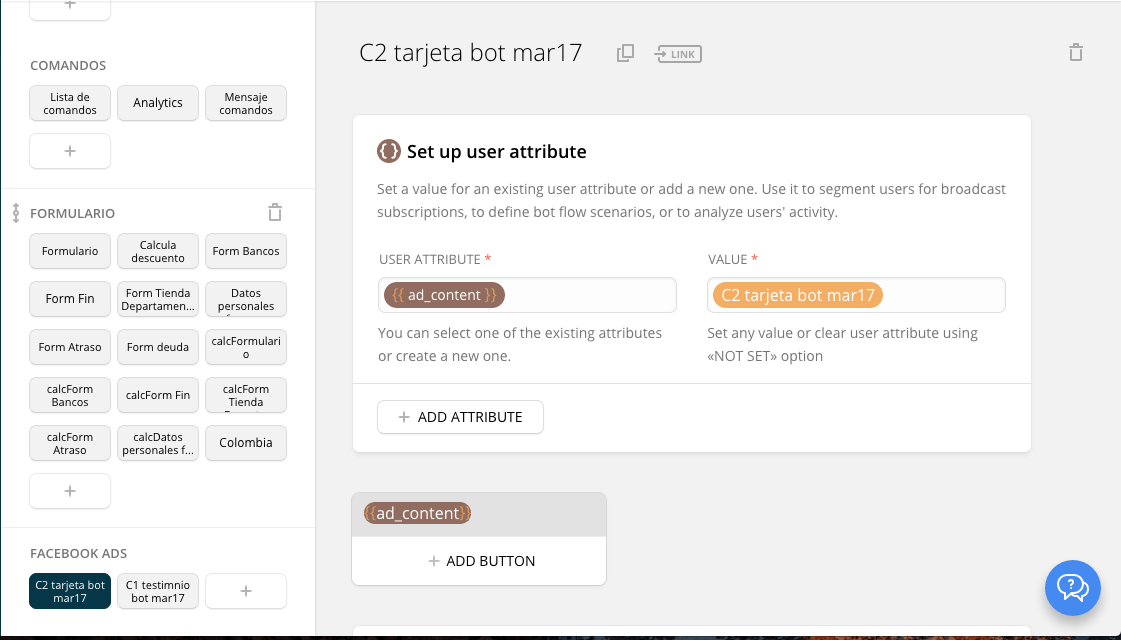
\includegraphics[width=\textwidth]{chatfuelFBAds.jpg}

Formulario - En esta sección está todo el proceso de captación de datos de contacto del usuario interesado en el producto.

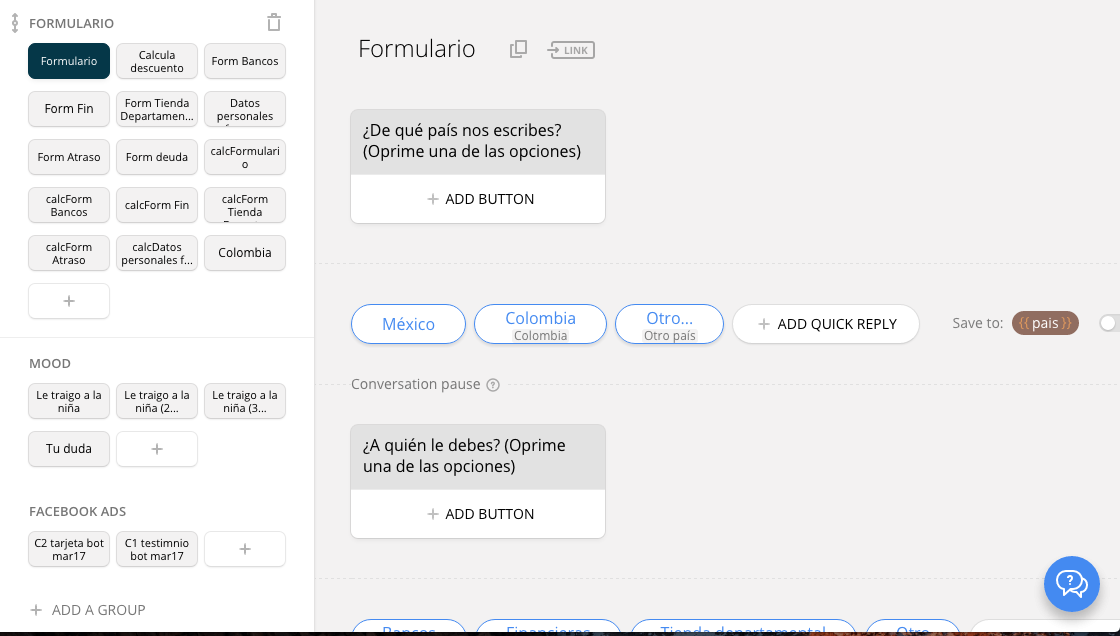
\includegraphics[width=\textwidth]{chatfuelFormulario.jpg}

\textbf{Cálculo de descuento, Formulario y Anuncios de Facebook}
Chatfuel funciona en este proyecto como el lugar para almacenar y crear la estructura del sistema que se presenta al usuario. Sin embargo, la funcionalidad requerida (hacer el cálculo de las cotizaciones, almacenar datos del usuario y datos de canales de adquisición de clientes) no es cubierta por la plataforma. Afortunadamente cuenta con conectores y APIs de integración a servicios externos. Por ello, se crearon integraciones y microservicios para las secciones de cálculo de descuento, formulario y anuncios de Facebook
\textbf{Flujo de cálculo de descuento y almacenamiento de datos}
Para hacer el cálculo del descuento se tenían que resolver dos cosas que no se pueden hacer directamente en Chatfuel. Hacer cálculos sobre datos insertados y almacenar datos en una base de datos. Por ello, se crearon dos micro servicios \textit{Lambda} \cite{kiran2015lambda}, \textbf{calculaDescuento} y \textbf{almacenaLeads}. Los cuales solucionan los dos aspectos faltantes de la herramienta.
Para acceder al micro servicio de \textbf{calculaDescuento} se utiliza un request GET con un query string que incluye los datos necesarios para el cálculo del descuento: deuda, banco, atraso de pago y si la persona ha pedido dejar sus datos ya. 
El servicio lo procesa y devuelve un mensaje con los datos insertados para el cálculo y el descuento resultante. Si el usuario aún no pide dejar sus datos se le invita a insertarlos para que un vendedor lo pueda contactar. 
El micro servicio \textbf{almacenaLeads} manda a través de un request POST los datos de contacto del usuario a la Base de datos: nombre completo, deuda, institución acreedora, atraso, e-mail, teléfono, campaña. Este servicio no genera ninguna respuesta al usuario.

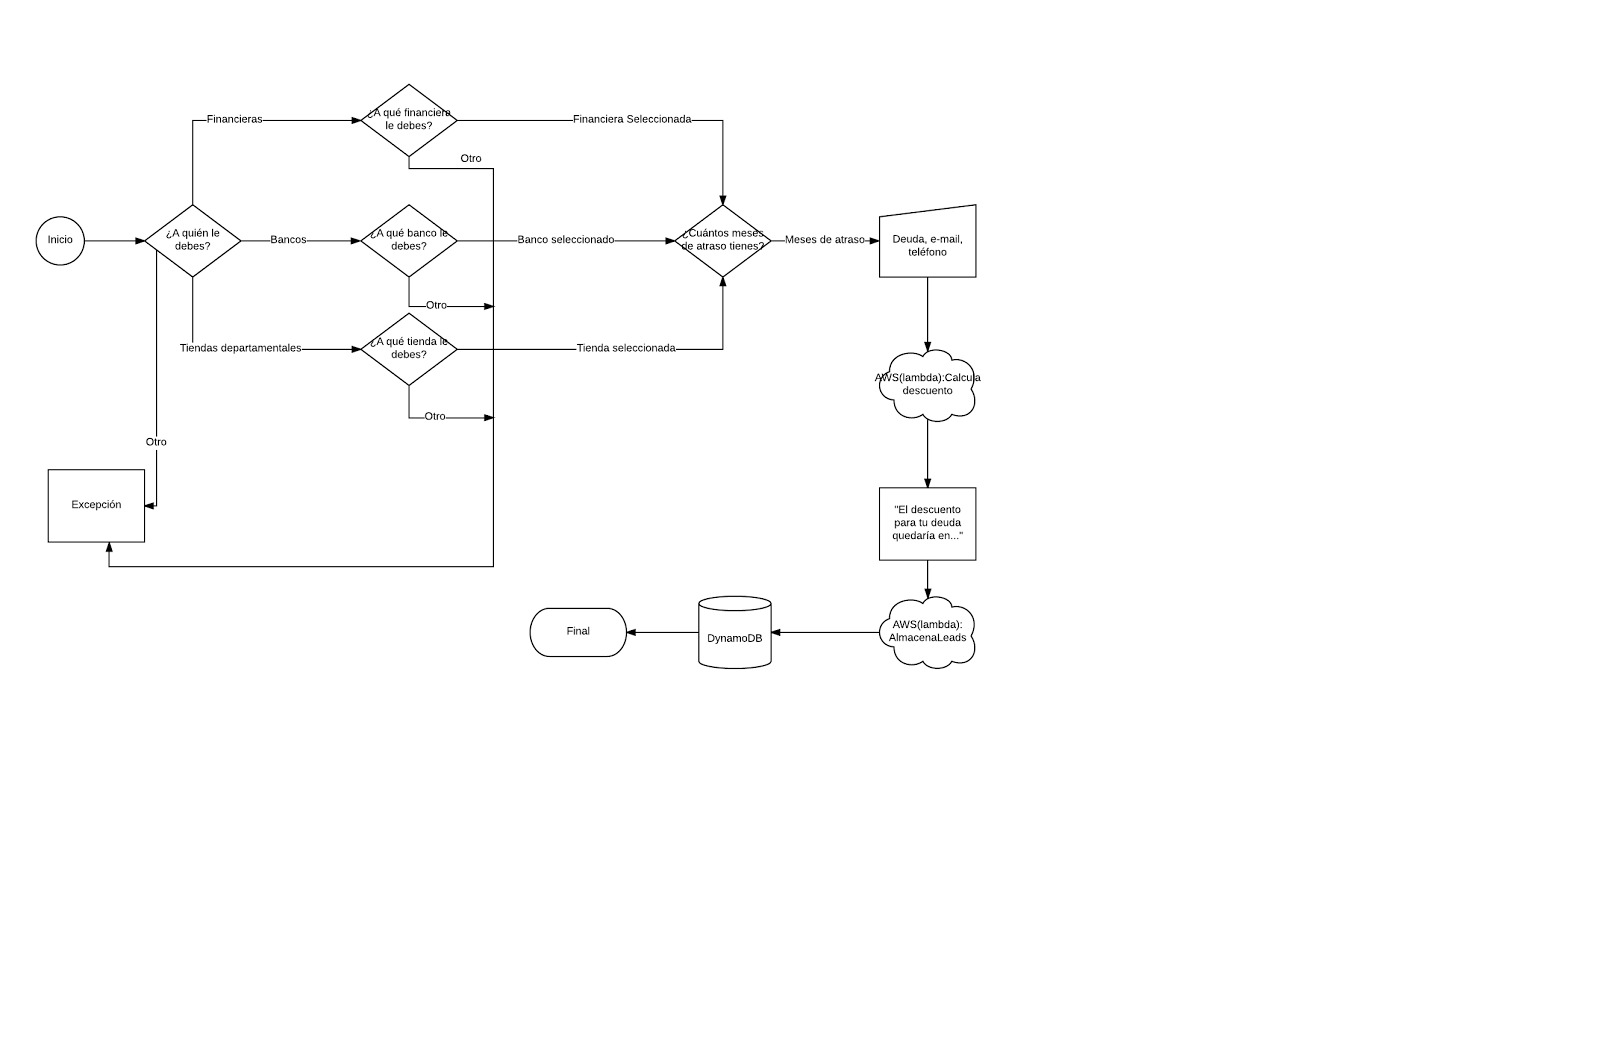
\includegraphics[width=\textwidth]{diagramaFlujoDatos.jpg}

\textbf{calculaDescuento}
La función recibe los datos que el bot le manda del usuario. Calcula el descuento a partir de la institución y meses que debe la persona. Estos valores fueron sacados de la forma en que se calcula el descuento en la página web promocional de Resuelve Tu Deuda; los cuales están basados en los promedios de los descuentos conseguidos por institución y meses de atraso.  Ese descuento se aplica a la deuda insertada y se calcula el monto final a pagar. Al final se regresa un objeto JSON con un mensaje indicando la deuda inicial, los meses de atraso, el porcentaje de descuento y el monto final estimado de su deuda si se hace cliente.
\textbf{almacenaLeads}
Para hacer la inserción al CRM, donde los vendedores ven los leads, se manda un POST a un endpoint que recibe los datos necesarios para hacer un registro nuevo (Nombre, teléfono, correo electrónico, meses de atraso, banco, system\_id, medio de contacto). Adicionalmente se añade una llave que asegura que el POST viene del bot.
\begin{itemize}
\item Se hacen un par de validaciones para verificar que los datos insertados sean válidos:
\item Se verifica que el correo tenga una terminación correcta de dominio (.com, .mx, etc) sino, se le añade ‘.com’ por default. Se verifica que ahora el formato sea correcto.
\item Se cambian todos los valores utf-8 a formato ascii
\item Se eliminan las comas presentes en los montos de deuda
\item Se transforma en un JSON
\item Y finalmente se envía a una función lambda que manda a Salesforce los nuevos leads.
\end{itemize}
El código detallado se encuentra en el apéndice

\textbf{Facebook Ads}
Una de la vía por la que más gente descubre a Resuelve es a través de los anuncios de Facebook. Por lo que se aprovechó esa ventaja para atraer gente a iniciar la conversación por esa vía también. Sin embargo, estos anuncios son pagados y deben ser monitoreados para que los costos por lead estén en los rangos esperados, así como el detalle de cual campaña tiene un mejor desempeño. Para solucionar esto se utilizó la estructura del objeto en JSON del mensaje mostrado al darle click a un anuncio que llevaba a Messenger. 
En la estructura del objeto JSON se utilizó la notación que utiliza Chatfuel para identificar los bloques que se deben mostrar y se asignó a cada anuncio un bloque de contenido. El cual consiste en una tarjeta que guarda en una variable el nombre de la campaña y redirige al usuario al mensaje de bienvenida (Figura 8). Para el usuario es un proceso transparente, sin embargo, el dato de la campaña se guarda en la base de datos si el usuario elige dejar sus datos de contacto.\cite{friedrich} 

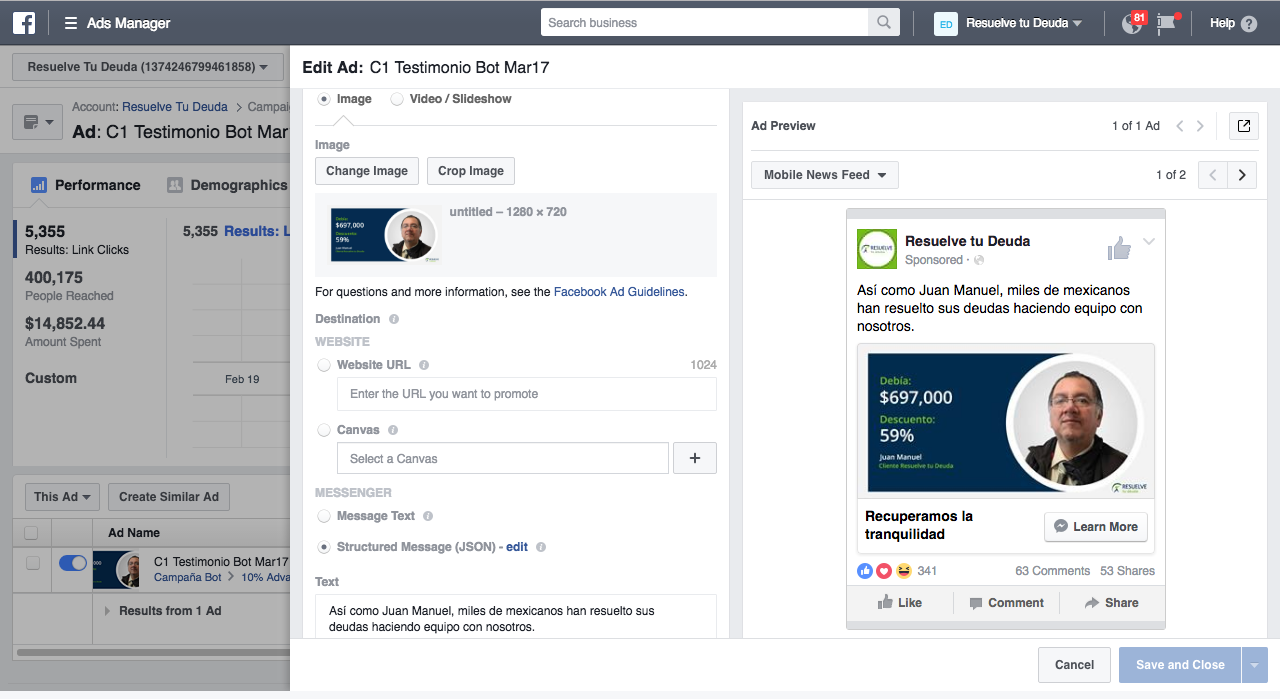
\includegraphics[width=\textwidth]{facebookAdsJSON.jpg}

\textbf{Procesamiento de Lenguaje Natural}
Los usuarios pueden conversar también a través de la introducción de frases con su teclado. Estas frases son interpretadas por el sistema de “AI” de Chatfuel, en donde se permite poner reglas, ejemplos de datos de entrada que armarán el modelo de procesamiento de lenguaje natural y la respuesta correcta como bloque de contenido o una respuesta corta de texto. Todo este procesamiento se hace con ayuda del algoritmo propietario de chatfuel.

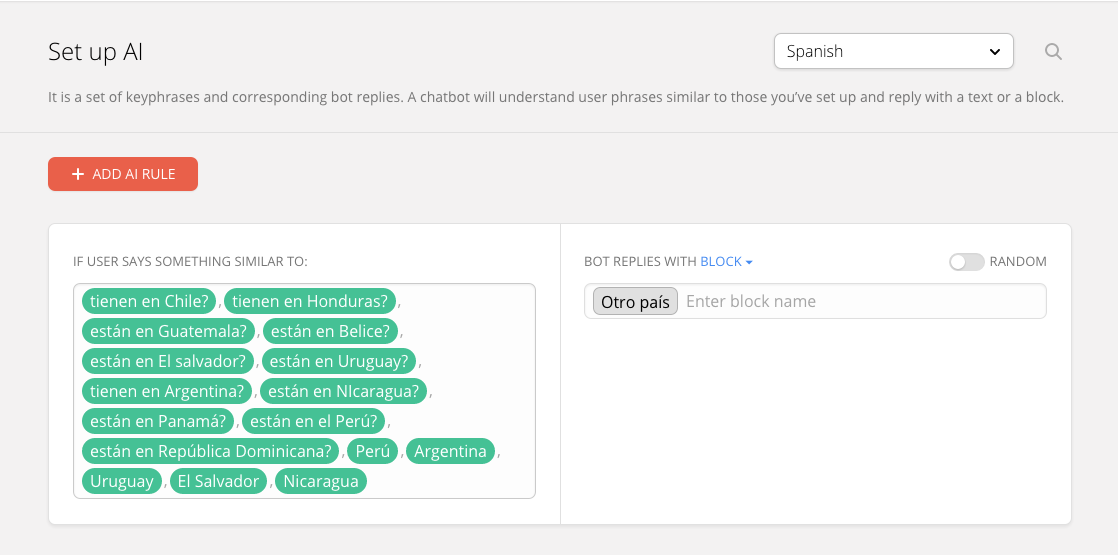
\includegraphics[width=\textwidth]{chatfuelAI.jpg}

Chatfuel recibe una consulta como datos de entrada. Con los datos trata de interpretar la consulta con la intención más adecuada en función de la información contenida (ejemplos, entidades utilizadas para anotaciones, contextos, parámetros, eventos) y el modelo de aprendizaje automático del agente, en este caso las reglas del chatbot. El algoritmo transforma el texto de la consulta en datos ejecutables y devuelve datos de salida como un objeto de respuesta JSON.


\chapter{Pruebas}
\textbf{Metodología}

Analizando los datos de interacción web se sabe que la gente que decide darnos sus datos lo hace el 90\% la primera vez que visita la página(figura 1 del apéndice).Entonces lo más acercado a la realidad sería tener a usuarios nuevos cada vez que se hagan pruebas.
Se realizaron pruebas antes del lanzamiento al público del chatbot. Se eligieron al azar 5 miembros del equipo de marketing, los cuales no tenían conocimiento alguno de la existencia del proyecto. La prueba consistió en decirles que el bot iba a poder atenderlos como si fueran una persona interesada en Resuelve tu deuda y contestar algunas preguntas sobre el producto. Cada individuo participó en una etapa diferente del desarrollo del bot. A continuación se muestran un transcrito de cada iteración de pruebas:

\textbf{Notación:}
\begin{itemize}
\item -  Individuo (“opniones del individuo”)
\item + Bot
\item *  Descripción de eventos en la plataforma
\end{itemize}



\textbf{Pruebas chatbot 1.0}


*Se muestran dos veces el mensaje de bienvenida

-COMO FUNCIONA EL PROGRAMA,

+ "te ayudamos a liquidar deudas que ya no puedes pagar con hasta 70\% de descuento. Nosotros negociamos con tus acreedores y ajustamos tus pagos mensuales a lo que puedas pagar "

- ”Es mucha información”

-como negocian las deudas? con que bancos?

+(Oops, no entendí eso . Intentalo de nuevo ¿Cómo te puedo ayudar?)

-como le hacen para negociar ?

+(Oops, no entendí eso . Intentalo de nuevo ¿Cómo te puedo ayudar?)

-tengo un límite de deuda?

+(Oops, no entendí eso . Intentalo de nuevo ¿Cómo te puedo ayudar?)

-quiero liquidar mis deudas

+¿A quién le debes? (Bancos) (Financieras) (Tiendas departamentales)

-Bancos

+¿A qué banco le debes?

*(AMEX) (BANAMEX) (BANORTE/IXE) (BBVA/BANCOMER) (HSBC) (INBURSA) (INVEX) (SANTANDER) (SCOTIABANK) (BANCO WALMART)

-AMEX

+¿Cuántos meses de atraso tienes?

*(0-5 meses) (6 meses) (7 meses) (8 meses) (9 meses) (10 o más meses)

-6 meses

+¿Cuánto debes en total?

-300000

+¿Cuál es tu correo?

-*****@resuelve.mx

+¿A qué número prefieres que te marquemos?


-1234567890

+Tu deuda de \$ 300000.0 con AMEX con atraso de
Quedaría con un 25 \% de descuento en \$ 225000.0
¡Gracias! Un asesor te contactará pronto

*Menú

\smallskip
\textbf{Observaciones y cambios para siguiente versión}
\smallskip
\textbf{[Etapa]}Principio del camino:


 \textbf{[Cambio]}Que se presente como un bot al principio y establecer expectativas a usuarios: 
Tienes que hablarle o el bot se introduce. 
Se tarda en contestar, establecer esa expectativa en el tiempo de respuesta.  Comunicar: "No es instantáneo, me tardo unos segundos".

\textbf{[Cambio]}
"Hola 'NAME' soy Resuelbot, un robot muy rápido y eficiente creado para ayudarte :), si no tengo una respuesta para tí uno de mis humanos te atenderá. Dime ¿En qué te puedo ayudar?".
\textbf{[Etapa]}Conoce el programa: El plan integral de ahorro no dice mucho.
Te ayudamos a liquidar deudas que ya no puedes pagar con hasta 70\% de descuento. Nosotros negociamos con tus acreedores y ajustamos tus pagos mensuales a lo que puedas pagar ;). 

\textbf{[Cambio]} Los sliders son iguales - quitar el segundo y cambiar el copy a ve nuestro video.

\textbf{[Cambio]} Cotización - se trabó cuando le di un input de texto en la opción múltiple de bancos. 

\textbf{[Cambio]} Ajustar el texto para preguntar “¿Cuál es tu deuda más grande?”

\textbf{[Etapa]}Cotización - no acepta entradas de texto en la opción múltiple de bancos.

\textbf{[Cambio]} Ajustar el texto para preguntar la deuda más grande

\textbf{[Cambio]}Por ahora, ser más claros en el copy añadiendo "no uses comas o signos".

\textbf{[Etapa]}Datos personales:

\textbf{[Cambio]} preguntar “A qué número prefieres que te marquemos?”
[Añadir]Algún horario en particular?

\textbf{[Etapa]}Menú al final de la cotización: 

\textbf{[Cambio]} En lugar de “no sé qué preguntar” cambiar por "Tengo otra pregunta"

\textbf{[Añadir]}Agregar a parte del "Quiero que me hablen" un "Quiero cotizar mi descuento".

\textbf{[Etapa]}Quiero saber más: Necesitamos generar confianza. Hay que dar una respuesta más  convincente: 

\textbf{[Cambio]}Resuelve Tu Deuda fue fundada por Javier y Juan Pablo en 2006, la primera reparadora de crédito en México! emoji: bandera mex y tarjeta -foto-. Hoy somos más de mil colaboradores resolviendo problemas de deuda, hemos ayudado a más de 80k clientes a recuperar su tranquilidad . -foto, footer "mira cuantos somos :o-

\textbf{[Cambio]} “Déjanos tus datos” cambiar por “Quiero una asesoría", tentativamente la gente todavía quiere saber más sobre el producto, suena muy agresiva la primera opción. 

\textbf{[Etapa]}Casos de éxito/testimonios

\textbf{[Cambio]}Hay que tener un copy de transición entre el input que sale de la opción múltiple "Estos son algunos de nuestros clientes y sus historias, conócelos"....Agregar a las opciones del bloque, menú.  

\textbf{[Etapa]}Sucursales

\textbf{[Cambio]}Cambiaría el copy a "encuentra la sucursal que más cerca te quede" o contáctanos por teléfono agregar la opción de teléfono o un botón que llame-> agregamos la cotización. Segunda versión podemos personalizar el bloque de cada zona para que no te lleve a la página general de sucursales. 
Testimonios-> punto 8.

\textbf{[Etapa]} Validación sobre el mínimo de deuda:
Agregar que tienes que estar atrasado y revisar el copy: "Los requisitos para entrar al programa Resuelve son: que estés atrasado en el pago de tus deudas, que tus deudas sumen más de \$35,000 pesos y que esas deudas sean con bancos, tiendas departamentales, Crédito Familiar o Credomatic.

\textbf{[Etapa]} Beneficios: las imágenes de los beneficios son de baja calidad, cambiarlas. " Estos son los beneficios del programa Resuelve:"
Conseguimos descuentos de hasta 70\% ;)
Nosotros nos encargamos de negociar con los bancos .
Atendemos las llamadas de cobranza.
Te damos asesoría legal y financiera gratis a lo largo de todo el programa Resuelve.
Empezamos a sanear tu Buró para que seas candidato a crédito en el futuro.
Total visibilidad del proceso de negociación y de repago a través de nuestra aplicación móvil.

\textbf{[Nueva Etapa]} Después del escenario de éxito hay que agregar un mensaje que pida un comentario para mejorar el bot- Después de cada cotización.

\textbf{[Mejoras]}Métricas. Qué vemos, cómo nos damos cuenta de en qué momento fallamos? 
\textbf{[Nueva opción]} Dar la opción para que pueda contestar un agente de servicio a cliente. 

\medskip
\textbf{Mejoras para la siguiente versión:}

Cambiar copies con la revisión previa
Guardar datos del formulario en una hoja de cálculo de en línea “Google Sheet”
Hacer cálculo de descuento y regresar el cálculo como respuesta

\medskip
\textbf{Pruebas chatbot 2.0}

Se hacen algunas modificaciones al flujo y mensajes del bot para mejorar la experiencia:
\begin{itemize}
\item Se añaden todas las mejoras comentadas en la prueba 1.0 
\item Se añaden algunos mensajes extra para hacer más natural el segundo saludo del bot.
\item Se alimenta a la lista de entradas diferentes saludos para hacer más robusta la interacción
\item Se da formato a los datos que se guardan en la BD

\end{itemize}

Se hicieron algunas pruebas con algunas personas que no estaban involucradas al proyecto pero son parte de la empresa.
Se les dijo que probaran el chatbot sin ninguna instrucción adicional. 
Fueron 10 personas. La mayoría optó por pedir más información acerca de la empresa, calcular el descuento sobre alguna deuda y dejar sus datos. 
Todos llegaron al mensaje por default, el cual indica que lo escrito no fue reconocido por el chatbot como una entrada esperada.
Se pidió proporcionar retroalimentación sobre la experiencia con el chatbot. Se recopilaron varias opiniones:
"Debería poder reconocer diferentes tipos de entradas cuando te pregunta sobre tu deuda"
"Hay algunas cosas que no me supo contestar que la gente usualmente tiene dudas antes de entrar al programa"
"Debería poder responder alguien si no entiende mi pregunta"
Se hacen algunos cambios al flujo para hacer más clara la interacción y limitaciones del chatbot:
Se añade a la lista de comandos la opción de hablar con una persona.
Se añade a la pila de entradas de reconocimiento de lenguaje natural frases como: "cuanto cobran?","
\medskip
\textbf{Pruebas chatbot 3.0}
Ahora se asocia el chatbot con el Fan Page de Resuelve Tu Deuda México y se le asigna a una persona que se encargue de responder a usuarios que pidan hablar con un humano.
Para hacer
Se observaron diversos tipos de interacción. Se agrupan las conversaciones en tres tipos:
-Nueva interacción
-Servicio a cliente
-Empleados (testers)
Con las nuevas interacciones se puede observar que siguen el flujo, van casi directo a pedir una cotización y dejar sus datos para un posterior contacto con un asesor. Se puede notar un nivel de satisfacción positivo
Las personas del grupo de servicio a cliente se le 
Hay que ver como segmentar a la gente que tiene mayor interacción. scoring
Se añade un typing en bloques largos i.e. "Quiero saber más"
Piden préstamos
deudas que no son suyas
cuando no está la Community Manager
Ser más claros con el tener que escoger una opción

\medskip
\textbf{Pruebas chatbot 4.0}
Varios se quedan a la mitad del camino a la hora de dejar sus datos

\medskip
\textbf{Pruebas chatbot 5.0}
Salen 2 ads que dirigen la conversación al bot [pedirle a Diego las imágenes]
Se añade la opción de decir de donde nos vista si no es de México o Colombia y se guarda en otra Hoja de Google Sheets
Se quita el mensaje que indica el monto mínimo si es menor la deuda a \$35,000

\thispagestyle{empty}

\chapter{Conclusiones}

Conluyo que...

%----------------------------------------------------------------------------------------
%	APÉNDICES
%----------------------------------------------------------------------------------------

\addtocontents{toc}{\vspace{2em}} % Agrega espacios en la toc

\appendix % Los siguientes capítulos son apéndices

%  Incluye los apéndices en el folder de apéndices

\chapter{Apéndice}
\section{bot.php}
Código que hace la inserción a CRM
\begin{minted}{php}
<?php
if(isset($_POST['chatfuel'])){
  if($_POST['chatfuel'] == "8cuNbZVtDgYJvkdzYbohnPiY"){
    $_POST['system_id'] = (int)$_POST['system_id'];
    /Translate/
    $_POST['first_name'] = $_POST['fb_first_name']." ".$_POST['fb_last_name'];
    $_POST['phone']     = str_replace(" ","",$_POST['phone']);
    $_POST['phone']     = substr($_POST['phone'],0,10);
    $_POST['landing'] = $_POST['ad_content'];
    $_POST['months_behind'] = str_replace(" meses","",$_POST['meses']);
    $_POST['borrower_insitute'] = $_POST['acredores'];
    $_POST['borrower_insitute'] = $_POST['acredores'];

    /Validation and fix/
    if(!preg_match('/./',$_POST['email'])){
        $_POST['email'] = $_POST['email'].'.com';
    }

    if(filter_var($_POST['email'], FILTER_VALIDATE_EMAIL)) {
    }else{
      $datetime = date("Y_m_d_H_i_s");
      $_POST['email'] = $datetime."@unknown-mail.com";
    }

    function toASCII( $str ){
        return strtr(utf8_decode($str), 
            utf8_decode(
            'ŠŒŽšœžŸ¥µÀÁ ÃÄÅÆÇÈÉÊËÌÍÎÏÐÑÒÓÔÕÖØÙÚÛÜÝßàáâãäåæçèéêëìíîïðñòóôõöøùúûüýÿ'),
            'SOZsozYYuAAAAAAACEEEEIIIIDNOOOOOOUUUUYsaaaaaaaceeeeiiiionoooooouuuuyy');
    }

    $_POST['email']       = toASCII($_POST['email']);
    $_POST['debt_amount'] = str_replace(",","",$_POST['debt_amount']);

    /Unset old values/
    unset($_POST['fb_first_name']);
    unset($_POST['fb_last_name']);
    unset($_POST['ad_content']);
    unset($_POST['meses']);
    unset($_POST['acredores']);
    unset($_POST['chatfuel']);

    /Transform to json/
    $data=json_encode($_POST);
    
    /Test or production/
    $url = 'https://urmdamghr3.execute-api.us-east-1.amazonaws.com/prod/Leads/registerLead';

    $ch = curl_init( $url );
    curl_setopt( $ch, CURLOPT_POST, 1);
    curl_setopt( $ch, CURLOPT_POSTFIELDS, $data);
    curl_setopt( $ch, CURLOPT_FOLLOWLOCATION, 1);
    curl_setopt( $ch, CURLOPT_HEADER, 0);
    curl_setopt( $ch, CURLOPT_RETURNTRANSFER, 1);

    $response = curl_exec( $ch );
  }
}
print_r("v0.3");
exit("");\end{minted}

\section{calculaDescuento.py}
Código que calcula el descuento de los clientes
\begin{minted}[mathescape,gobble=2]{python}
  # coding: utf-8
from __future__ import print_function
import json
import sys
import boto3


print('Loading function')

#event={"institucion": sys.argv[1],"deuda":sys.argv[2],"atraso":sys.argv[3]}
ins=event['institucion']
deuda=round(float((event['deuda'])))
atraso=int(event['atraso'])
descuento=0



def lambda_handler(event, context):    
    """Ejecuta el cálculo del descuento
    Argumentos:
    event -- datos del usuario para cálculo del descuento(dict)
    context --  variables de entorno(str)"""
    print("Parametros recibidos: ")
    print("Institucion= "+ins)
    print("Deuda= " + str(deuda))
    print("Atraso= "+str(atraso))
    
    nuevodescuento=calculaDescuento(ins,atraso)
    print ("Nuevo Descuento="+ str(nuevodescuento))

    nuevadeuda = round(deuda*.01*nuevodescuento)
    print("Nueva deuda="+str(nuevadeuda))
    #nuevadeuda=calculaDescuento(ins,deuda,atraso)
    mensaje1='Tu deuda de $'+ str(deuda)+' con ' +ins+" con atraso de "+ str(atraso)+" meses"
    mensaje2='Quedaria en $'+ str(nuevadeuda)
    print(mensaje1)
    print(mensaje2)

    not_encoded=[{"text": mensaje1},{"text": mensaje2}]
    res=json.dumps(not_encoded)
    
    return(not_encoded)







"""Métodos para calcular descuento
Argumentos:
atraso: meses de atraso(int)"""
descuento=0
def descuentoBancomer(atraso):
    if atraso==1:
            descuento=15
    elif atraso==2:
            descuento=32
    elif atraso==3:
            descuento=48
    elif atraso==4:
            descuento=60
    elif atraso==5:
            descuento=67
    elif atraso>=6:
            descuento=85
    return descuento

def descuentoBanamex(atraso):
    if atraso>=0 and atraso<=4:
        descuento=0
    elif atraso==5:
        descuento=57
    elif atraso==6:
        descuento=62
    elif atraso==7:
        descuento=66
    elif atraso==8 or atraso==9:
        descuento=70
    elif atraso>=6:
        print (str(atraso) +" es mayor a 6")
        descuento=74
        print("entonces descuento="+str(descuento))
    return descuento

def descuentoAmex(atraso):
    if atraso>=0 and atraso<=2:
        descuento=0
    elif atraso==3:
        descuento=5
    elif atraso>=4:
        descuento=25
    return descuento

def descuentoBanorte(atraso):            
    if atraso>=0 and atraso<=4:
        descuento=5
    elif atraso>=5 and atraso<=8:
        descuento=40
    elif atraso>=9:
        descuento=55
    return descuento

def descuentoHSBC(atraso):
    if atraso>=0 and atraso<=2:
        descuento=0,
    elif atraso>=3 and atraso<=4:
        descuento=40,
    elif atraso>=5 and atraso<=6:
        descuento=50,
    elif atraso>6:
        descuento=60
    return descuento

def descuentoScotiabank(atraso):
    if atraso>=0 and atraso<=4:
        descuento=0,
    elif atraso>4:
        descuento=45
    return descuento
def descuentoGlobal(atraso):
    if atraso>=0 and atraso<=4:
        descuento=0
    elif atraso>4:
        descuento=45
    return descuento

def descuentoInbursa(atraso):
    if atraso>=0 and atraso<=4:
        descuento=45
    elif atraso>4:
        descuento=50
    return descuento 



def descuentoCA(atraso):
    if atraso>=1 and  atraso<=4:
        descuento=0
    elif atraso>4:
        descuento=10
    return descuento

def descuentoIxe(atraso):
    if atraso<5:
        descuento=0
    elif atraso>=5:
        descuento=30
    return descuento

def descuentoInvex(atraso):
    if atraso>=0 and atraso<=2:
        descuento=0
    elif atraso==3:
        descuento=35
    elif atraso>=4:
        descuento=45
    return descuento

def descuentoCredFamiliar(atraso):
    if atraso >=1 and atraso<=4: 
        descuento=0
    elif atraso>=5:
        descuento=35
    return descuento

def descuentoSantander(atraso):
    if atraso==1:
         descuento=10
    elif atraso==2:
        descuento=20
    elif atraso==3:
        descuento=30
    elif atraso==4:
        desceunto=50
    elif atraso>=5:
        descuento=55
    return descuento

def descuentoSantander(atraso):
    if atraso==1:
        descuento=10
    elif atraso==2:
        descuento=20
    elif atraso==3:
        descuento=30
    elif atraso==4:
        desceunto=50
    elif atraso>=5:
        descuento=55
    return descuento

def descuentoPH(atraso):
    if atraso>4:
        descuento=15
    return descuento

def descuentoSears(atraso):
    if atraso>4:
        descuento=15
    return descuento

def descuentoCredomatic(atraso):
    if atraso >=1 and atraso<=4:
        descuento=0
    elif atraso>=5 and atraso<=6:
        descuento=10
    elif atraso>6:
        descuento=20
    return descuento

def descuentoWalmart(atraso):
    if atraso>=1 and atraso<=4:
        descuento=0
    elif atraso>=5 and atraso<=6:
        descuento=10
    elif atraso>6:
        descuento=20
    return descuento
def descuentoLiverpool(atraso):
    if atraso>=1 and atraso<=4:
        descuento=0
    elif atraso>=5 and atraso<=6:
        descuento=10
    elif atraso>6:
        descuento=20
    return descuento

def calculaDescuento(ins, atraso):
    """calcula el total a pagar con el descuento
    Argumentos:
    ins -- institucion a la que se le debe(str)
    atraso -- meses pago atrasado(int)"""
    switcher = {
            "Bancomer": descuentoBancomer(atraso),
            "Banamex": descuentoBanamex(atraso),
            "AMEX": descuentoAmex(atraso),
            "Banorte":descuentoBanorte(atraso),
            "HSBC":descuentoHSBC(atraso),
            "Scotiabank":descuentoScotiabank(atraso),
            "Global":descuentoGlobal(atraso),
            "Inbursa":descuentoInbursa(atraso),
            "Liverpool":descuentoLiverpool(atraso),
            "C&A":descuentoCA(atraso),
            "IXE":descuentoIxe(atraso),
            "Invex":descuentoInvex(atraso),
            "Credito Familiar":descuentoCredFamiliar(atraso),
            "Santander":descuentoSantander(atraso),
            "Palacio de Hierro":descuentoPH(atraso),
            "Sears":descuentoSears(atraso),
            "Credomatic":descuentoCredomatic(atraso),
            "Walmart":descuentoWalmart(atraso),
             2: lambda: "two",
    
        }
    func = switcher.get(ins, lambda: "nothing")
    
    # Execute the function
    return func



lambda_handler(event,1)

\end{minted}
\chapter{Imagenes} 
Time Lag - días desde que se produce la primera interacción hasta que se produce la conversión
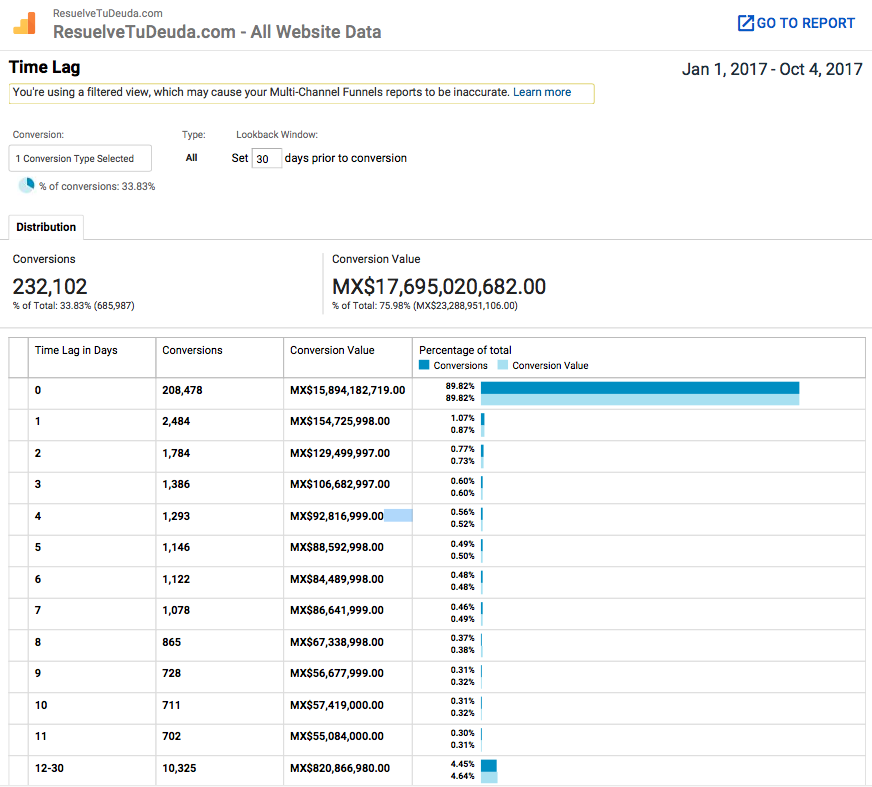
\includegraphics[width=\textwidth]{TimeLag.jpg}

%\thispagestyle{empty}
%\include{Apendices/AppendixB}
%\include{Apendices/AppendixC}

\addtocontents{toc}{\vspace{2em}} % Agrega espacio en la toc


%----------------------------------------------------------------------------------------
%	BIBLIOGRAFÍA
%----------------------------------------------------------------------------------------

\bibliographystyle{plain}
\bibliography{bibliografia.bib}


%\printbibliography
\end{document}